\documentclass[10pt]{beamer}

\setbeamertemplate{note page}[default]
%\setbeameroption{hide notes}
\setbeameroption{show notes}


\usetheme[progressbar=frametitle]{metropolis}
\usepackage{appendixnumberbeamer}

\usepackage{booktabs}
\usepackage[scale=2]{ccicons}

\usepackage{pgfplots}
\usepgfplotslibrary{dateplot}
\usepackage{multicol}
\setlength{\columnsep}{1.5cm}

\usepackage{animate}
\usepackage{lmodern}
\usepackage[T1]{fontenc}
\usepackage{mathtools}
\usepackage{graphicx}
\usepackage{caption}
\usepackage[export]{adjustbox}

\definecolor{set1}{RGB}{228, 26, 28}
\definecolor{set2}{RGB}{77, 175, 74}
\definecolor{set3}{RGB}{255, 127, 0}
\definecolor{set4}{RGB}{166, 86, 40}
\definecolor{set5}{RGB}{153, 153, 153}

\usepackage{xspace}
\newcommand{\themename}{\textbf{\textsc{metropolis}}\xspace}

\newcommand\Fontvi{\fontsize{8}{9}\selectfont}
\newcommand\Fontvr{\fontsize{6}{7}\selectfont}

\setbeamerfont{parent A}{size=\small}


\title{Exploratory Data Analysis}
\subtitle{Digital Transformation of Healthcare}
% \date{\today}
\date{}
\author{Michoel Snow M.D. Ph.D. and Glen Ferguson Ph.D.}
\institute{Center for Health Data Innovations}
% \titlegraphic{\hfill\includegraphics[height=1.5cm]{logo.pdf}}

\begin{document}

\maketitle

\section{Exploratory Data Analysis}

\begin{frame}{Bioinformatics Pipeline}
	\begin{center}
		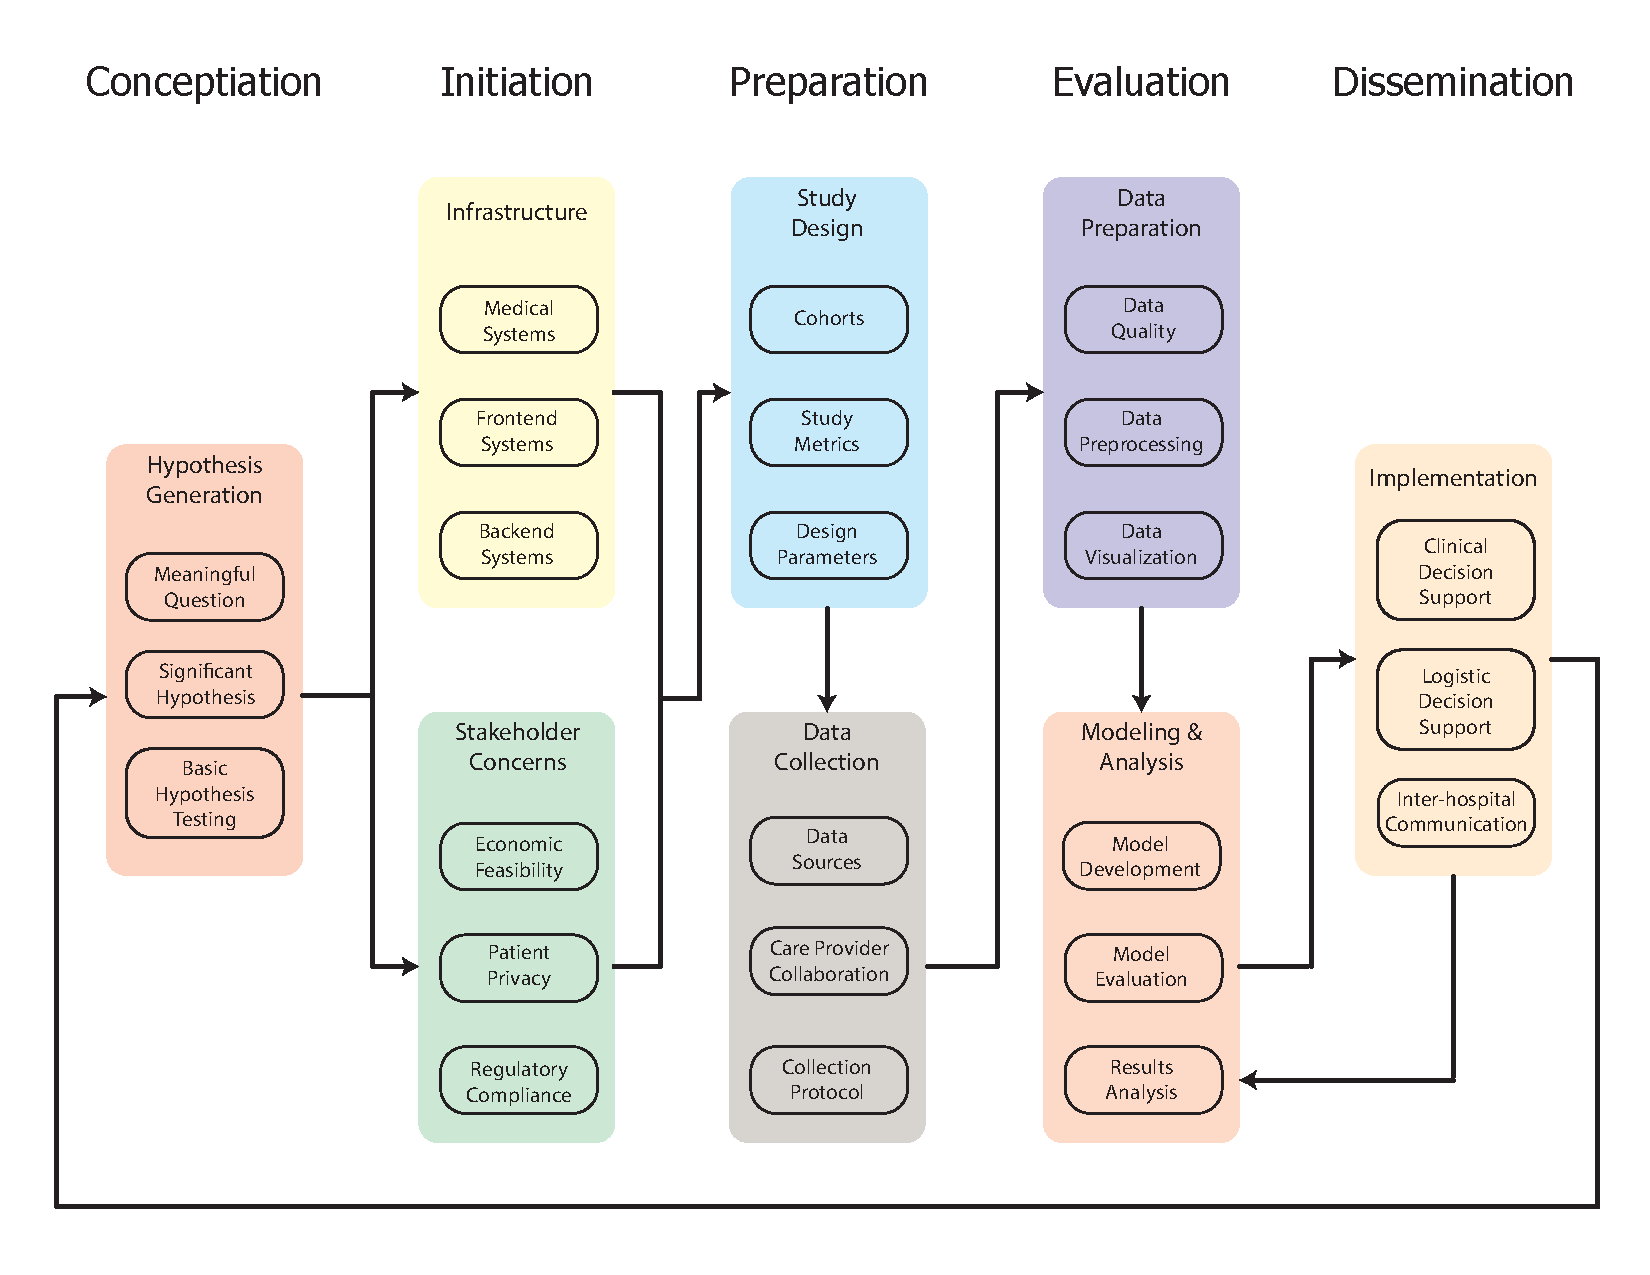
\includegraphics[width=0.8\textwidth]{images/informatics_pipeline.pdf}	
	\end{center}
\end{frame}


\begin{frame}{Data Analysis}
	\begin{center}
		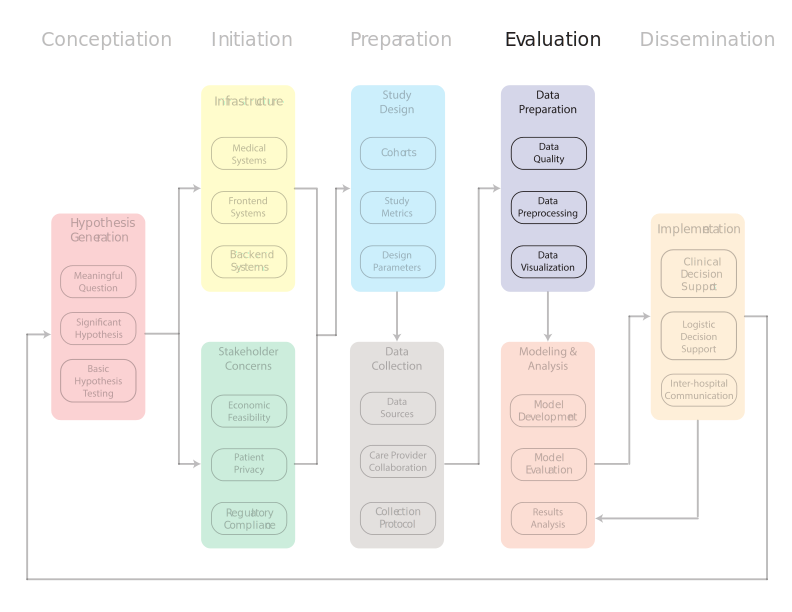
\includegraphics[width=0.8\textwidth]{images/informatics_pipeline_evaluation.pdf}
	\end{center}
\end{frame}

\begin{frame}{EDA}
	\begin{itemize}
		\item Objectives
			\begin{itemize}
				\item Define EDA
				\item Know the purpose of EDA
				\item Understand a visualization toolbox
				\item Ask questions about data using EDA
			\end{itemize}
	\end{itemize}
\end{frame}

\begin{frame}{What is EDA?}  
	\begin{itemize}
		\item EDA
			\begin{itemize}
			    \pause
				\item An method of summarizing the main points of a data set, most often using visualization
				\pause
				\item Distinct from other types of analysis for confirming or validating hypotheses
				\pause
				\item Used to find hidden structure in the data, e.g., unknown relations between the variables or correlation with the target variable
			\end{itemize}
	\end{itemize}
\end{frame}

\begin{frame}{Why visualize?}
Why not just use summary statistics?
	\pause
	\begin{figure}	
		\caption{Anscombe's Quartet}
		\includegraphics[width=0.9\textwidth, center, trim=0cm 0cm 0 0cm]{images/anscombe.png}
	\end{figure}
\end{frame}

\begin{frame}{Why perform EDA?}  
	\begin{itemize}
		\item EDA
			\begin{itemize}
			    \pause
				\item Assess data quality
				\pause
				\item Understand the types of data in the data set
					\begin{itemize}
						\item Continuous
						\item Time Series
						\item Categorical
						\item Boolean (T/F)
						\item Low Cardinality (few categories)
						\item High Cardinality (few categories)
					\end{itemize}
				\pause
				\item Determine the parameters of the data set
					\begin{itemize}
						\item Min, max, median, and percentiles of numerical data
						\item Distribution of the numerical data
						\item Count, number of unique values, most common value, and frequency of most common values for categorical values
						\item Range and rolling values of a time series
					\end{itemize}
				\pause
				\item Develop hypothesis
				\pause
				\item Determine what prepossessing and modeling are appropriate
			\end{itemize}
	\end{itemize}
\end{frame}

\begin{frame}{Summary Stats}  
Summary Stats on Appt. Attendance Data Set
	\begin{table}[]
	\begin{tabular}{llll}
    		 & ApptTime  & LeadDays   & PatientAge \\
		mean & 11.663151 &  44.736143  &  44.722064  \\
		std  &  2.299348 &  35.997952  &  22.396794  \\
		min  &  8.100000 &  -3.000000  &   0.000000  \\
		25\% &  9.500000 &  15.000000  &  26.000000  \\
		50\% & 11.100000 &  35.000000  &  46.000000  \\
		75\% & 14.000000 &  70.000000  &  62.000000  \\
		max  & 16.300000 & 369.000000 & 104.000000
	\end{tabular}
\end{table}

%	\begin{figure}	
%		\caption{Non-linear Regression, {\tiny By Alexeicolin - Own work, CC BY-SA 3.0}}
%		\includegraphics[width=0.9\textwidth, center, trim=0cm 0cm 0 0cm]{images/%Isotonic_regression.pdf}
%	\end{figure}
\end{frame}

\begin{frame}{Summary Stats}  
Summary Stats on Appt. Attendance Data Set
\begin{table}[]
\begin{tabular}{llllllllllll}
 & ApptMonth & ApptDays & AppointmentBlock & \\
count & 21451 & 21451 & 21451 & \\
unique & 12 & 5 & 5 &  \\
top & May & Tue & None & \\
freq & 2023 & 4971 & 20932 & 
\end{tabular}
\end{table}
\end{frame}

\begin{frame}{Visualization Toolbox}
Univariate exploration
	\begin{figure}	
		\caption{Distributions of continuous variables}
		\includegraphics[width=1.1\textwidth, center, trim=0cm 0cm 0 0cm]{images/numerical_distributions.png}
	\end{figure}
\end{frame}

\begin{frame}{Visualization Toolbox}
Univariate exploration
	\begin{figure}	
		\caption{Counts of discreet variables}
		\includegraphics[width=1.1\textwidth, center, trim=0cm 0cm 0 0cm]{images/cat_columns.png}
	\end{figure}
\end{frame}

\begin{frame}{Visualization Toolbox}
Bivariate exploration
	\begin{figure}	
		\caption{Pair plot of continuous variables}
		\includegraphics[width=0.6\textwidth, center, trim=0cm 0cm 0 0cm]{images/pair_plot.png}
	\end{figure}
\end{frame}

\begin{frame}{Visualization Toolbox}
Bivariate exploration
	\begin{figure}	
		\caption{Box plots discrete-continuous variables}
		\includegraphics[width=0.6\textwidth, center, trim=0cm 0cm 0 0cm]{images/boxplot_days.png}
	\end{figure}
\end{frame}



\begin{frame}{Visualization Toolbox}
Bivariate exploration
	\begin{figure}	
		\caption{Box plots discrete-continuous variables}
		\includegraphics[width=0.6\textwidth, center, trim=0cm 0cm 0 0cm]{images/boxplot_appt_time.png}
	\end{figure}
\end{frame}

\begin{frame}{Visualization Toolbox}
Bivariate exploration
	\begin{figure}	
		\caption{Box plots discrete-continuous variables}
		\includegraphics[width=0.6\textwidth, center, trim=0cm 0cm 0 0cm]{images/boxplot.png}
	\end{figure}
\end{frame}

\begin{frame}{Visualization Toolbox}
Bivariate exploration with target 
	\begin{figure}	
		\caption{Pair plot with groups indicated}
		\includegraphics[width=0.65\textwidth, center, trim=0cm 0cm 0 0cm]{images/pair_plot_groups.png}
	\end{figure}
\end{frame}

\begin{frame}{Visualization Toolbox}
Bivariate exploration with target 
	\begin{figure}	
		\caption{KDE Plot of variable with target groups}
		\includegraphics[width=0.65\textwidth, center, trim=0cm 0cm 0 0cm]{images/kde_age_target.png}
	\end{figure}
\end{frame}

\begin{frame}{Visualization Toolbox}
Bivariate exploration with target 
	\begin{figure}	
		\caption{Count plot with target}
		\includegraphics[width=0.65\textwidth, center, trim=0cm 0cm 0 0cm]{images/count_bar_NewToProv_target.png}
	\end{figure}
\end{frame}

\begin{frame}{Visualization Toolbox}
Bivariate exploration with target
	\begin{figure}	
		\caption{Counts of discreet variables}
		\includegraphics[width=0.65\textwidth, center, trim=0cm 0cm 0 0cm]{images/count_bar_Weekday_target.png}
	\end{figure}
\end{frame}

\begin{frame}{Visualization Toolbox}
Feature Selection
	\begin{figure}	
		\caption{Relationship between the variables and the target}
		\includegraphics[width=0.65\textwidth, center, trim=0cm 0cm 0 0cm]{images/num_feature_corr_target.png}
	\end{figure}
\end{frame}

\begin{frame}{Visualization Toolbox}
Other Visualizations
	\begin{figure}	
		\caption{Covariance between variables}
		\includegraphics[width=0.65\textwidth, center, trim=0cm 0cm 0 0cm]{images/rank2d_covariance.png}
	\end{figure}
\end{frame}

\begin{frame}{Visualization Toolbox}
Other Visualizations
	\begin{figure}	
		\caption{Radial plot to determine variable separability}
		\includegraphics[width=0.65\textwidth, center, trim=0cm 0cm 0 0cm]{images/radviz.png}
	\end{figure}
\end{frame}

\begin{frame}{Visualization Toolbox}
Other Visualizations
	\begin{figure}	
		\caption{PCA with axis plotted}
		\includegraphics[width=0.65\textwidth, center, trim=0cm 0cm 0 0cm]{images/pca_biplot_3d.png}
	\end{figure}
\end{frame}

\begin{frame}{Visualization Toolbox}
Other Visualizations
	\begin{figure}	
		\caption{Parallel coordinate plot}
		\includegraphics[width=0.65\textwidth, center, trim=0cm 0cm 0 0cm]{images/normalized_sampled_parallel_coordinates.png}
	\end{figure}
\end{frame}

\end{document}